\chapter*{Appendix E: Design Alternatives}
\label{appendix:design_alternatives}
\addcontentsline{toc}{chapter}{Appendix E: Design Alternatives}

\section*{E.1 Rejected Visualisation Primitives}
\label{sec:solution:viz:alt}

Six visualisation primitives were considered for one or more charts in
the catalogue and rejected. Table~\ref{tab:viz:rejected} records each
rejection with the applicable chart and the specific reason.

\begin{table}[!htbp]
  \centering
  \caption{Visualisation primitives considered and rejected.}
  \label{tab:viz:rejected}
  \footnotesize
  \renewcommand{\arraystretch}{1.25}
  \begin{tabularx}{\linewidth}{p{3.0cm} X X}
    \hline
    \textbf{Primitive} & \textbf{Where it might have applied} & \textbf{Reason for rejection} \\
    \hline
    Pie chart & Any composition view (fare class, payment channel, company share) & Compares angles poorly and saturates above five slices; ranked bar conveys composition more directly \cite{knaflic2015}. \\
    Three-dimensional bar chart & Any quantitative comparison & Three-dimensional effects distort length and area perception, leading to systematic misreading of magnitudes \cite{knaflic2015}. \\
    Choropleth keyed to districts & Boarding density across the city & Districts vary substantially in area and confound population density with administrative geometry; replaced by hexagonal-bin map \cite{h3}. \\
    Word cloud & Any categorical-label summary (route names, stop names) & Encodes magnitude through font size, which is a poor visual channel for quantitative comparison and offers no axis for inspection. \\
    Dendrogram & Cross-route clustering on the Demand and Crowding theme & Forces a hierarchical reading on the routes that the underlying feature space does not support; replaced by the route constellation (chart~1.3). \\
    Radial axis (radar plot) & Per-route multi-metric summary & Each radar chart shows one route only, defeating cross-route comparison; the route constellation (chart~1.3) and the per-stop box plot (chart~6.4) carry the multi-metric reading more readably. \\
    \hline
  \end{tabularx}
\end{table}

Three rejections are illustrated on actual project data. A pie on
the five fare-class categories (student cash, student smartcard,
regular cash, regular smartcard, free-fare) cannot be visually
ordered; the ranked horizontal bar of Figure~\ref{fig:viz:reject_pie}
makes the rank order immediately readable.

\begin{figure}[!htbp]
\centering
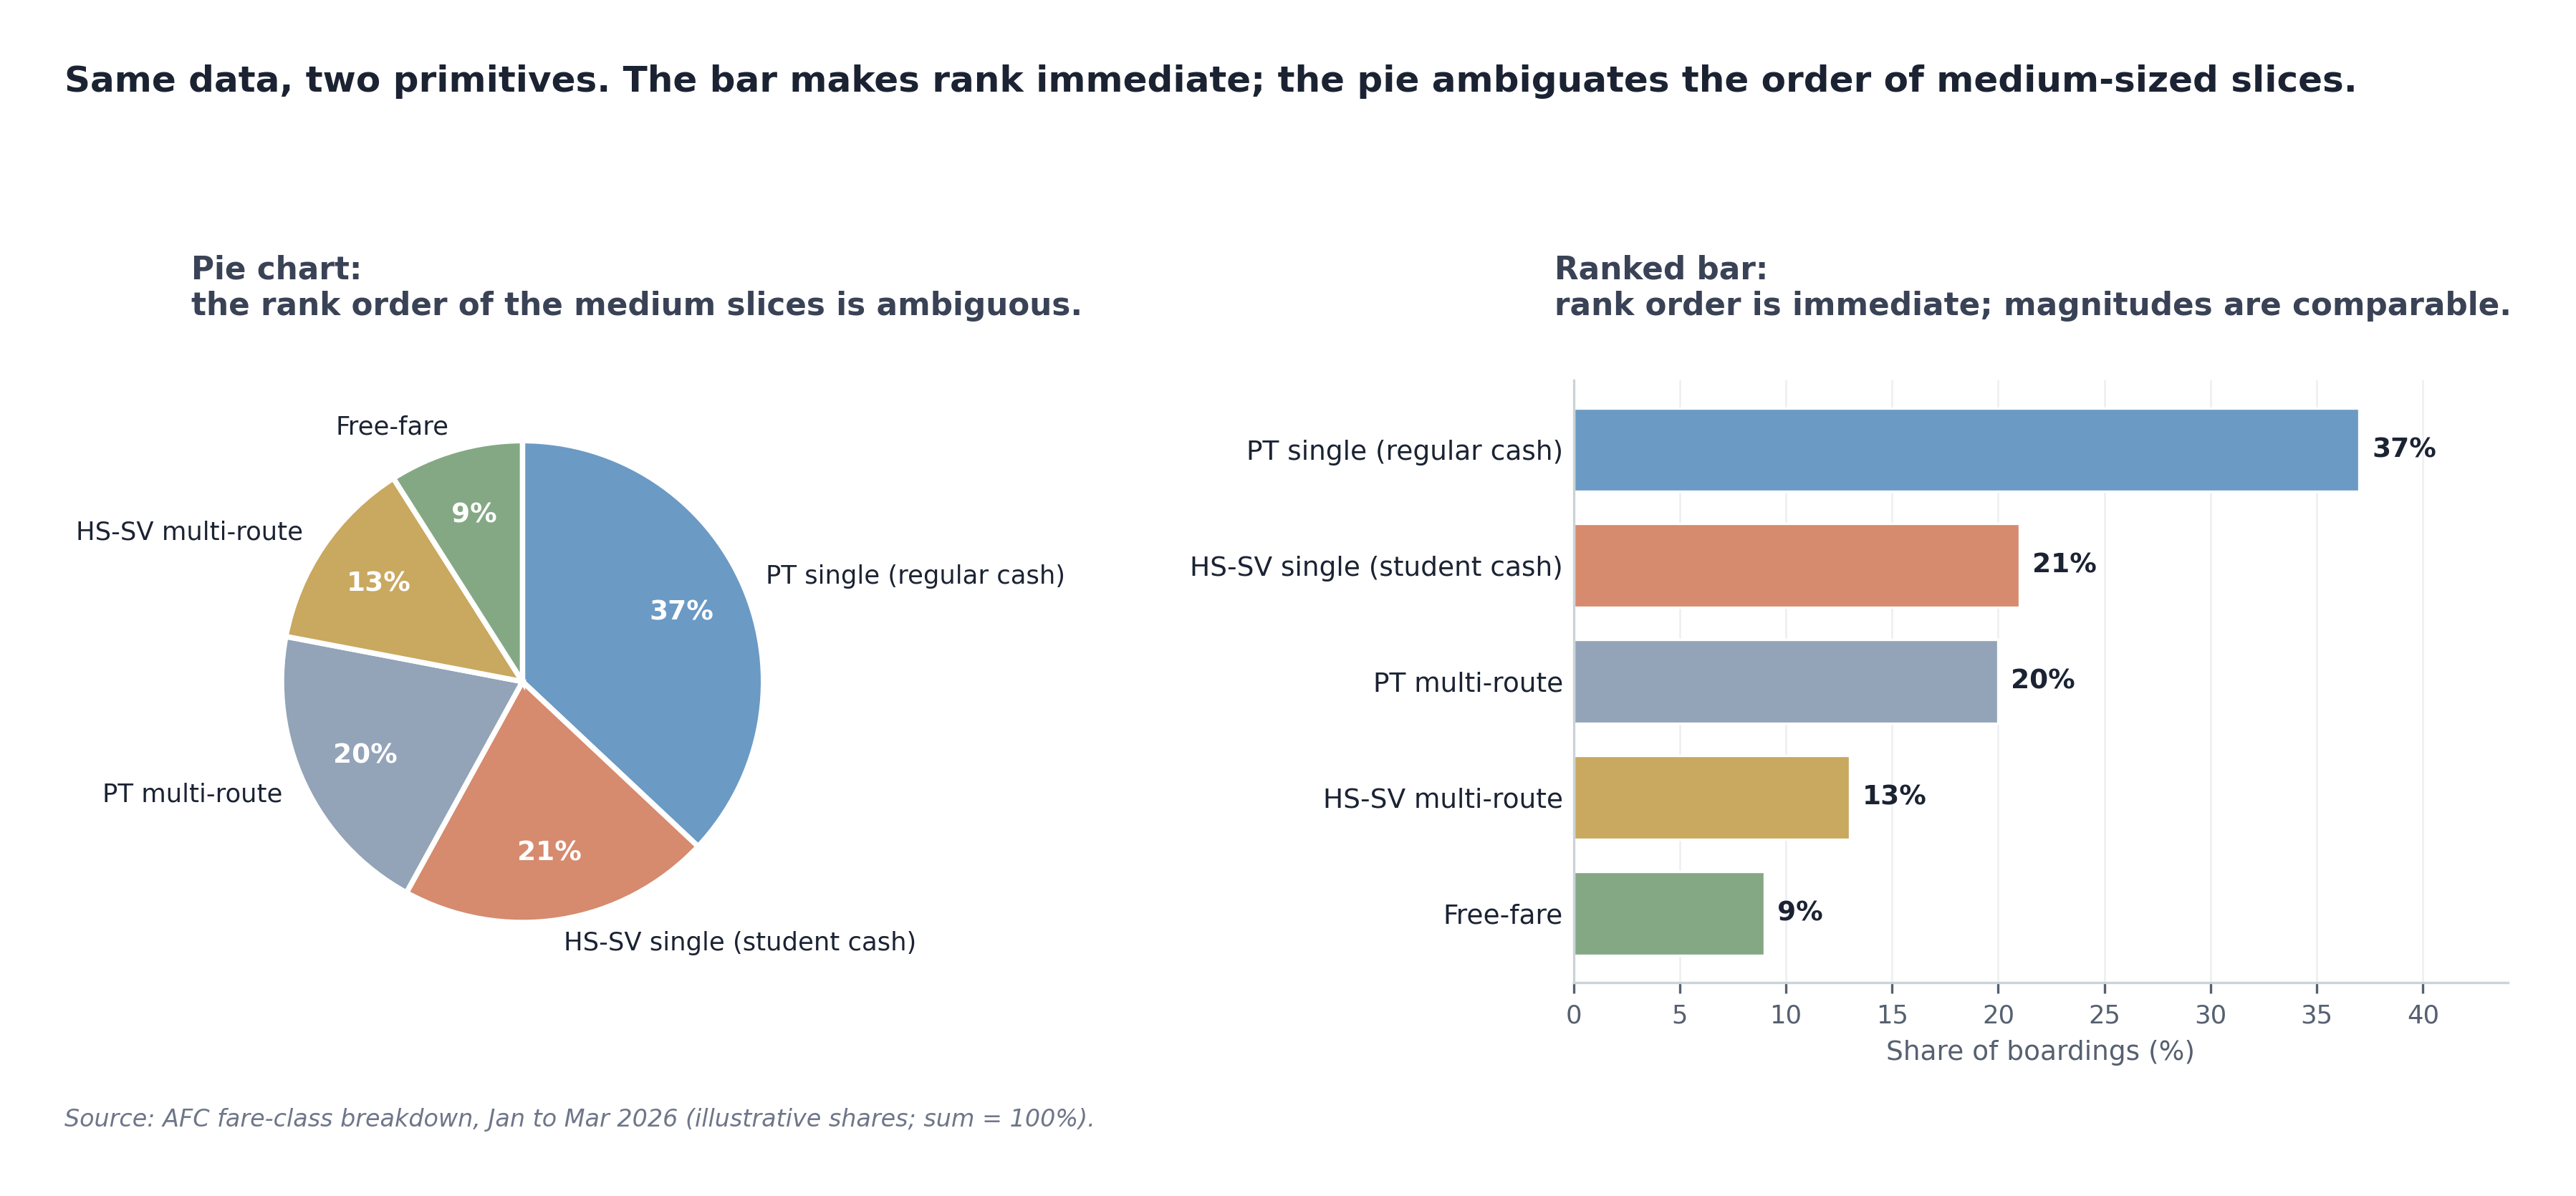
\includegraphics[width=0.92\linewidth]{images/diagrams/solution_reject_pie_vs_bar.png}
\caption{Pie chart versus ranked horizontal bar on the same fare-class breakdown.}
\label{fig:viz:reject_pie}
\end{figure}

Ho Chi Minh City's twenty-four urban districts vary in area by more
than an order of magnitude; a choropleth confounds boarding intensity
with administrative area. Figure~\ref{fig:viz:reject_choropleth}
contrasts a district choropleth with the hexagonal-bin equivalent at
500-metre cells, which is uniform in area.

\begin{figure}[!htbp]
\centering
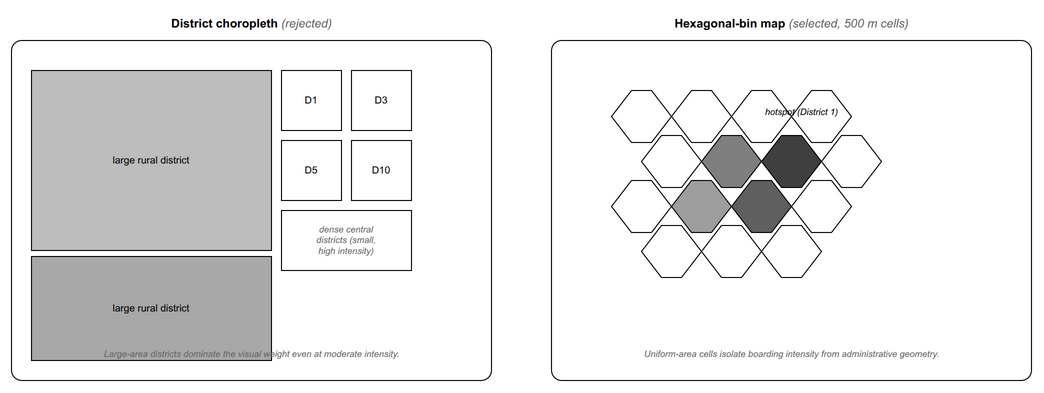
\includegraphics[width=0.96\linewidth]{images/diagrams/solution_reject_choropleth_vs_hex.png}
\caption{District choropleth versus hexagonal-bin map.}
\label{fig:viz:reject_choropleth}
\end{figure}

A dendrogram imposes a strict tree hierarchy on the route feature
space (peak hours, student share, weekend drop, length, company),
which does not exhibit hierarchical structure. The route constellation
(chart~1.3) encodes the same archetype membership through a bubble
scatter without inventing merge heights.

\section*{E.2 Rejected Interaction Patterns}
\label{sec:solution:interaction:rejected}

Four interaction patterns were considered and rejected in favour of
the click-to-entity-detail panel composition described in
Section~\ref{sec:solution:interaction}.

\noindent\textbf{Multiple Coordinated Views with simultaneous cross-chart brushing.}
The original direction inherited from the literature
survey~\cite{liu2022,heer2012interactive}. Rejected after the user
interface shell was finalised: the shell renders one chart per canvas
at any time, so simultaneous re-renders across sibling charts would be
invisible to the reader. Implementing propagation against invisible
state expends complexity with no perceptible analytical gain.

\noindent\textbf{Full-page navigation model.}
Each chart occupies its own URL; the browser back-button is the
primary navigation surface. Rejected because cross-chart coordination
cannot be expressed through page transitions; the reader would lose
the theme-scoped selection on every navigation.

\noindent\textbf{Modal-dialog entity-detail.}
Clicking an entity opens a modal overlay rather than a side panel.
Rejected because the modal blocks the analytical surface beneath it
and forces the reader to dismiss the modal before consulting any other
chart; the side panel keeps the chart canvas visible behind the panel
at reduced opacity.

\noindent\textbf{Whole-application linked-brushing.}
A selection in any chart propagates to every chart in every theme.
Rejected for the same reason as MCV-simultaneous (no visible target
charts) and additionally because it grows the implementation surface
superlinearly in the catalogue size.
